% Nikolai Nielsens "Fysiske Fag" preamble
\documentclass[a4paper,10pt]{article} 	% A4 papir, 10pt størrelse
\usepackage[english]{babel}
\usepackage{Nikolai} 					% Min hjemmelavede pakke
\usepackage[dvipsnames]{xcolor}

% Margen
\usepackage[margin=1in]{geometry}

% Max antal kolonner i en matrix. Default er 10
%\setcounter{MaxMatrixCols}{20}

% Hvor dybt skal kapitler labeles?
%\setcounter{secnumdepth}{4}	
%\setcounter{tocdepth}{4}


% Hvilket nummer skal der startes med i sections? (n-1)
%\setcounter{section}{0}	

% Til nummerering af ligninger. Så der står (afsnit.ligning) og ikke bare (ligning)
\numberwithin{equation}{section}


% Header
%\usepackage{fancyhdr}
%\head{}
%\pagestyle{fancy}

%Titel
\title{Numerical Methods in Physics Week 2}
\author{Nikolai Plambech Nielsen}
\date{}

\begin{document}
	\maketitle
	\section{Diffusion}
	For this assignment, diffusion from an initial delta-function peak is evaluated numerically. The differential equation is the diffusion equation, which in one dimension is
	\begin{equation}\label{key}
		\diff{C}{t} = D \diff{^2 C}{t^2}
	\end{equation}
	where $ D $ is the diffusion constant. This is a partial differential equation which necessitates the use of other methods. For evaluating the time derivative, simple Euler integration can be used, but for evaluating the double space derivative, a new method is used. First, space needs to be discretized, which allows one to calculate the derivative similarly to Euler integration. The integration scheme is called Forward in Time Centered in Space (FTCS), which for this equation uses 3 points at the last time step, to compute the value at each point in the next time step. To evaluate the $ j $'th point in space, the $ j-1 $'th, $ j $'th and $ j+1 $'th point, all from the last time step, is used. Numerically this is
	\begin{equation}
		C^{n+1}_j = C^n_j + \frac{D \Delta t}{h^2} (C^n_{j-1}+C^n_{j+1} - 2 C^n_j),
	\end{equation}
	where $ h $ is the distance between each point in space, equivalent to $ \Delta t $ in time.
	
	To numerically evaluate the delta-function, the following numerical equivalent is used
	\begin{equation}\label{key}
		\delta(x-x_0) \to \begin{cases}
		1/h & x = x_0 \\
		0 & x \neq 0,
 		\end{cases}
	\end{equation}
	as this is a sharp peak around $ x_0 $ and "integrating" this over all space gives 1:
	\begin{equation}\label{key}
		\sum \delta(x-x_0) h = \sum_{x_0}^{x_0} \frac{h}{h} = 1
	\end{equation}
	For simplicity, $ x_0 = 0 $ is used for all the following assignments. The analytical solution to this problem is
	\begin{equation}\label{key}
		C(x,t) = \frac{1}{\sigma(t) \sqrt{2\pi}} \exp\pp{-\frac{(x-x_0)^2}{2\sigma(t)}}, \quad \sigma(t) = \sqrt{2Dt}.
	\end{equation}
	which is a delta function in the limit of $ t\to 0 $, but spreads out as time passes.
	
	However, the choice of $ N $ might pose a small problem, if the $ x $-interval is centred around $ x=0 $. If there is an odd number of points, the middle-most point will definitely be $ x=0 $, but if there is an even number of points, this is not the case. $ x = 0 $ will lie directly between two points. To prevent any discrepancy, the delta-function is modified for even values of $ N $:
	\begin{equation}\label{key}
	\delta(x-x_0) \to \begin{cases}
	1/2h & x=x_0\pm h/2 \\
	0 & \text{otherwise}
	\end{cases}, \ (\text{for equal } N).
	\end{equation}
	
	To compare the numerical and analytical solutions, the following values are used: $D = 0.1, L = 2\pi,N=128 $, with $ h=L/(N-1) $ as this is the spacing MATLAB uses with the \texttt{linspace} function, and $ \Delta t = h^2/4D $. The positions after $ t = 1 $ are plotted, along with the difference between the two solutions
	\begin{figure}[H]
		\centering
		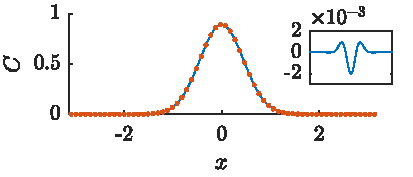
\includegraphics[width = 0.5\linewidth]{diffSimple.pdf}
		\caption{The numerical (blue line) and analytical (orange points) solutions to the diffusion equation for a delta function initial condition. An inset of the difference between the numerical and analytical solutions is also shown.}
		\label{fig:diffSimple}
	\end{figure}
	The analytical and numerical solution to the differential equation are in agreement, with a max difference of $ 2.04\D10^{-3} $. However, at the edges of the simulation, where both solutions are approximately zero, the fractional error does exceed 0.5 at places.
	
	Next the relation between error, grid size and time step size is explored. However, comparing errors between simulations with different grid sizes becomes difficult, as this does not allow for easy plotting. Therefore the error on the final time step is summed up and divided by the number of points to normalize the error. First the simulation is run with 128 points, for 1 unit of time, with 100 linearly spaced values of $ \Delta t $ between $ \Delta t_0 = h^2/2D $ and $ h^2/100D $. Next the simulation is run with between 20 and 1000 points in increments of 20, with $ \Delta t = h^2/4D $, where $ h = L/(N-1) $, to satisfy the stability condition. The results are shown in the figures below:
	 
	\begin{figure}[H]
		\centering
		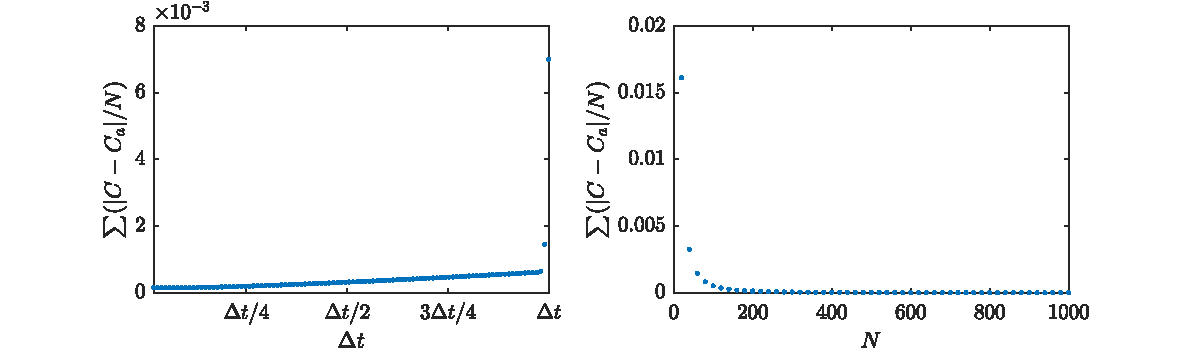
\includegraphics[width = \linewidth]{diffErr.pdf}
		\caption{Plots of the normalized cumulative error as a function of the time step size $ \Delta t $ (left) and grid size $ N $ (right). On the right plot, the grid size is $ N = 128 $, and on the left plot, the time step is $ \Delta t = h^2/4D $.}
		\label{fig:diffErr}
	\end{figure}
	The dependence on $ \Delta t $ seems approximately linear from $ \Delta t =  \Delta t_0$ to $ \Delta t = 8\Delta t_0/10 $, before becoming approximately constant. The first part is as expected, however the second is not. I do not know, if I have run into any limit to the accuracy of the simulation, or if my definition of error has anything to do with the result.
	
	The dependence on $ N $ is fully polynomial between in the chosen range, with a degree of roughly -2. This seems to corroborate with the expectation that the error in goes as $ O(h^2) = O(N^{-2})$.
	


	\subsection{von Neumann stability}
	The von Neumann stability condition is a method of determining the stability of a numerically simulated problem. To derive this, a trial function is inserted into the integration scheme for the problem, and the ratio of amplitudes between timesteps is isolated. The trial function is that of a complex standing wave:
	\begin{equation}\label{key}
		C_{\text{trial}}(x,t) = A(t) e^{ikx} \to C_j^n = A^n e^{ikjh}
	\end{equation}
	where $ n $ is the index in time, $ k $ is the wave number, $ j $ is the index in space and $ h $ is the grid spacing. The ratio $ \xi = A^{n+1}/A^{n} $ is then isolated in the integration scheme, and if $ |\xi| \leq 1 $, then the solution is stable. For this problem one gets
	\begin{equation}\label{key}
		A^{n+1} e^{ikjh} = A^n e^{ikjh} + \frac{D \Delta t}{h^2} (A^n e^{ik(j-1)h}+A^n e^{ik(j+1)h}-2A^n e^{ikjh})
	\end{equation}
	And upon dividing by $ A^n e^{ikjh} $ this becomes
	\begin{equation}\label{key}
		\xi = \frac{A^{n+1}}{A^n} = 1 + \frac{D \Delta t}{h^2} (e^{-ikh}+e^{ikh}-2) = 1 + \frac{D \Delta t}{h^2} (2\cos kh -2) = 1 - \frac{4D \Delta t}{h^2} \sin^2 kh/2.
	\end{equation}
	where Eulers formula and the trigonometric identity $ \sin^2(x) = (1-\cos(2x))/2 $ are used. Now, $ \sin^2 kh/2 $ oscillates between 0 and 1, and the constants $ D,\Delta t,h$ are all real and positive. This means that $ \xi \leq 1 $ for all values of the constants. But it might still be less than -1 for certain values of the constants. The worst case scenario is when $ \sin^2 kh/2 = 1 $, where the condition becomes
	\begin{equation}\label{key}
		-1 \leq 1-\frac{4D\Delta t}{h^2} \Rightarrow 2 \geq \frac{4D\Delta t}{h^2} \Rightarrow \Delta t \leq \frac{h^2}{2D}.
	\end{equation}
	which is the Von Neumann stability condition for this numerical integration scheme. To test this, the simulation is run with $ \Delta t = (1\pm 10^{-2}) \frac{h^2}{2D}$, or a 1\% deviation from the von Neumann limit in each direction:
	\begin{figure}[H]
		\centering
		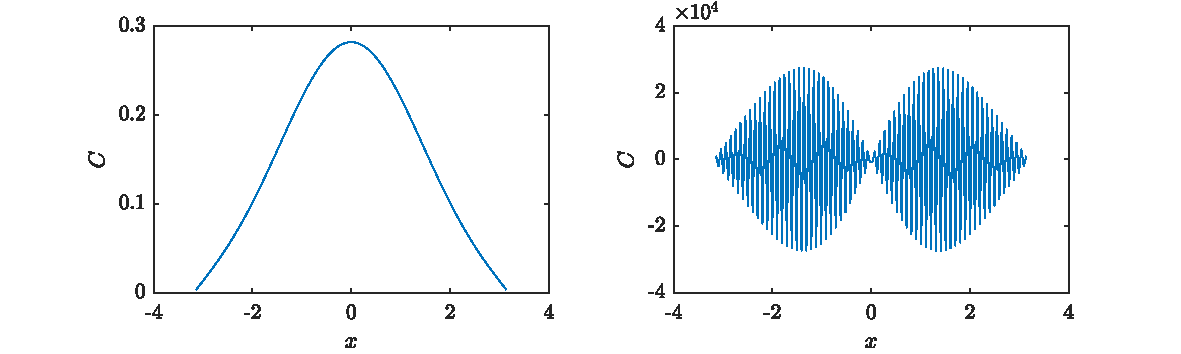
\includegraphics[width=\linewidth]{vonNeumann1.pdf}
		\caption{Plots of the numerical solutions to the simple diffusion problem, with $ \Delta t \approx h^2/2D $. Both are plotted at $ t = 10 $. On the left $ \Delta t = 0.99\D(h^2/2D) $ and on the right $ \Delta t = 1.01\D(h^2/2D) $.}
		\label{fig:von1}
	\end{figure}
	As seen, for $ \Delta t < \Delta t_0 $ the simulation runs as expected, but for $ \Delta t > \Delta t_0 $ (even by just 1\%) the result blows up.



	\section{Diffusion with constant source and decay}
	In this problem, two new terms are added to the differential equation: a decay term and a constant source term:
	\begin{equation}\label{key}
		\diff{C}{t} = S \delta(x-x_0) + D \diff{^2 C}{x^2}- \frac{C}{t}
	\end{equation}
	where the analytical solution at steady state is
	\begin{equation}\label{key}
		\frac{C(x)}{C(x_0)} = e^{-\frac{|x-x_0|}{\sqrt{\tau D}}}.
	\end{equation}
	
	For this exercise both FTCS and a new method, called the Spectral Method, will be used. The Spectral Method uses discrete Fourier Transformation to convert a PDE to an ODE, allowing the use of simple Euler integration, and then just inverse Fourier transformation at the desired timestep. Now, due to the way MATLAB handles its discrete Fourier Transforms, only even values of $ N $ can be used. Because of this, the source point $ x_0 = x_{N/2} $ is chosen, which has the value $ x_0 = -h/2 $.
	
	Furthermore, Fourier transforming a delta-function results in a complex wave $ e^{-ikx_0} $, and for some reason (maybe because the "wave number" is $ x_0 = -h/2 $), this causes the spectral method to explode for any $ \Delta t $ (even $ \Delta t = 5\D10^{-4}\D \Delta t_0 $, for the new value of $ \Delta t_0$ in this problem). To combat this, a different initial condition is used: a not too sharply peaked Gaussian function. This is an appropriate approximation, as the delta function can be defined as the limit of the Unitary Gaussian for $ \sigma \to 0 $. In practice the following is used
	\begin{equation}\label{key}
		\delta (x-x_0) \to \frac{1}{h} \exp\pp{-\frac{(x-x_0)^2}{10^{-2}}}.
	\end{equation} 
	This will of course give a larger error when comparing the numerical and analytical solutions, as they no longer solve the same problem.
	
	\subsection{von Neumann stability}
	The new integration scheme is
	\begin{align}\label{key}
		C^{n+1}_j &= C_j^n+ \Delta t \pp{S\delta(x-x_0) + \frac{D}{h^2}(C_{j-1}^n+C_{j+1}^n-2C_j^n) -\frac{C_j^n}{\tau}} \\
		&= \frac{D\Delta t}{h^2} (C_{j-1}^n+C_{j+1}^n) + \pp{1-\frac{\Delta t}{\tau} - 2\frac{D\Delta t}{h^2}}C_j^n + S\Delta t \delta(x-x_0).
	\end{align}
	where the delta function term is, in essence, an initial condition. For this reason, it is discarded in deriving the stability condition. This then becomes:
	\begin{equation}\label{key}
		A^{n+1} e^{ikjh} = A^n e^{ikjh}+ \Delta t A^n \pp{\frac{D}{h^2}(e^{ik(j-1)h}+e^{ik(j+1)h}-2e^{ikjh}) -A^n \frac{e^{ikjh}}{\tau}}.
	\end{equation}
	and isolating $ \xi $ gives
	\begin{equation}\label{key}
		\xi = \frac{A^{n+1}}{A^n} = 1 - \frac{4D \Delta t}{h^2} \sin^2(hk/2)- \frac{\Delta t}{\tau}
	\end{equation}
	where again Eulers formula and the trigonometric identity has been used. This is again always smaller than 1, but the worst case scenario of $ \sin^2(hk/2) = 1 $ gives
	\begin{equation}\label{key}
		2 \geq \Delta t \pp{\frac{4 D}{h^2}+\frac{1}{\tau}} \Rightarrow \Delta t \leq \frac{2\tau h^2}{4D\tau + h^2}.
	\end{equation}
	and with the same conditions as before ($ \Delta t = (1\pm 10^-2) \Delta t_0 $, end at $ t=10 $), the results are
	\begin{figure}[H]
		\centering
		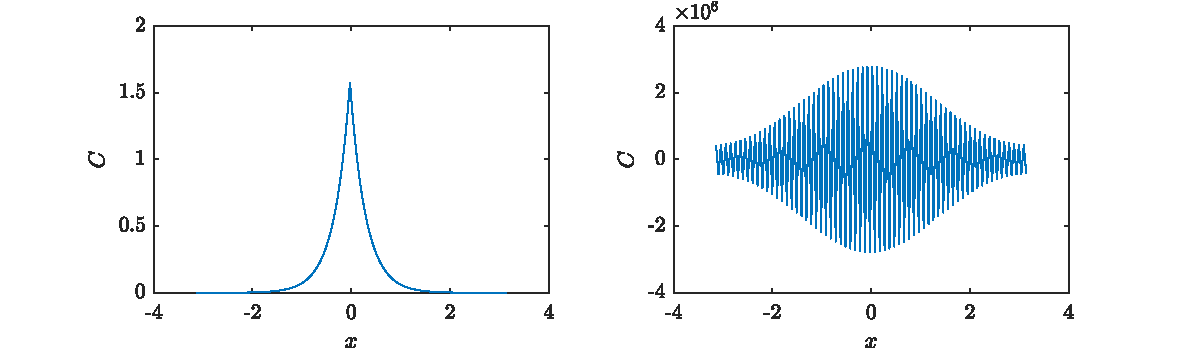
\includegraphics[width = \linewidth]{vonNeumann2.pdf}
		\caption{Plots of the numerical solutions to the simple diffusion problem, with $ \Delta t \approx \Delta t_0 $. Both are plotted at $ t = 10 $. On the left $ \Delta t = 0.99 \Delta t_0 $ and on the right $ \Delta t = 1.01 \Delta t_0 $.}
		\label{fig:von2}
	\end{figure}
	And just as before, the results are as expected.
	
	\subsection{Comparing the analytical solution and FTCS method}
	The analytical and numerical solution is compared as before, with $ \Delta t = \Delta t_0/2 $ and $ N=128 $. The results are plotted for $ t = 1 $:
	\begin{figure}[H]
		\centering
		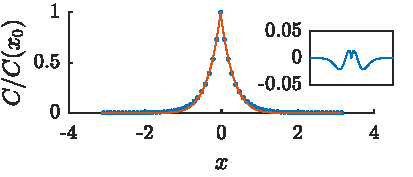
\includegraphics[width = 0.5\linewidth]{diffSource.pdf}
		\caption{The numerical (blue line) and analytical (orange points) solutions to the diffusion equation with a constant source and decay. An inset of the difference between the numerical and analytical solutions is also shown.}
		\label{fig:diffSource}
	\end{figure}
	For this problem the maximal fractional error is 2.16\%, even at the tails, which is much better than the almost 50\% for the simple diffusion problem.
	
	\subsection{The Spectral Method}
	\subsubsection{An example}
	The spectral method utilizes the fact that Fourier transforming a differential equation converts it to an algebraic equation in the inverse space. Namely, the $ n $'th derivative of an (at least) $ n $ times differentiable function (where it is assumed that the function and all derivatives vanish at infinity) becomes $ (ik)^n $ times the function. So:
	\begin{equation}\label{key}
		\diff{u(x)}{x} \to ik u(k), \quad \diff{^2u(x)}{x^2} = -k^2 u(k).
	\end{equation}
	As an example, the sum of the first and second derivative of $ \cos(2x) $ is calculated using this method. Analytically this is $ -4\cos(2x) -2 \sin(2x) $. The function is plotted in the interval $ x \in [-\pi,\pi] $, with $ N=128 $. The numerical and analytical solutions are plotted below:
	\begin{figure}[H]
		\centering
		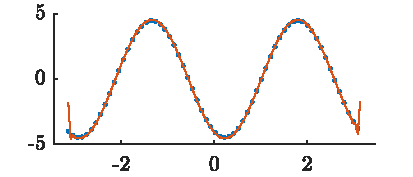
\includegraphics[width = 0.5\linewidth]{spectralEx.pdf}
		\caption{The numerically calculated sum of the first and second derivative of $ \cos(2x) $ (orange) and the analytical (blue points). Solved using the spectral method for $ N=128 $.}
		\label{fig:spectralEx}
	\end{figure}
	The numerical and analytical solutions are in agreement, except at the edges. This is due to the value of the function not going to zero at the edges, which means that the Fourier transformed function in reality is the desired function modulated by a square function, which changes the Fourier transform.
	
	\subsubsection{Solving the diffusion equation}
	
	
	
\end{document}

